\documentclass[10pt, sigconf]{acmart}

\usepackage{booktabs} % For formal tables

\usepackage{url}
%\usepackage[sort,space]{cite}
\usepackage{tabularx}
%\usepackage{algorithm2e}
\usepackage[ruled,vlined]{algorithm2e}
\usepackage{algpseudocode}
\usepackage{amsmath}
\usepackage{mathtools}
\newtheorem{mydef}{Definition}
\usepackage{rotating}
\usepackage{wrapfig}
\long\def\comment#1{}
\usepackage{multirow}
\usepackage{lscape}
\usepackage{stmaryrd}
\usepackage{wrapfig}
\usepackage{hhline}
\usepackage{textcomp,booktabs}
\usepackage{epstopdf}

\usepackage{graphicx}
\usepackage{subfig}
\usepackage[font=bf]{caption}

%\usepackage[draft]{hyperref}
\usepackage{hyperref}

\hypersetup{
  pdfstartview=FitH,
  pdfpagelayout=SinglePage,
  colorlinks=true,      % false: boxed links; true: colored links
  linkcolor=blue,       % color of internal links
  citecolor=magenta,    % color of links to bibliography
  filecolor=cyan,       % color of file links
  urlcolor=red          % color of external links
}

\usepackage{array}
\newcolumntype{L}[1]{>{\raggedright\let\newline\\\arraybackslash\hspace{0pt}}m{#1}}
\newcolumntype{C}[1]{>{\centering\let\newline\\\arraybackslash\hspace{0pt}}m{#1}}
\newcolumntype{R}[1]{>{\raggedleft\let\newline\\\arraybackslash\hspace{0pt}}m{#1}}

\newcommand{\bbR}{\mathbb{R}}
\newcommand{\calN}{\mathcal{N}}
\newcommand{\calR}{\mathcal{R}}
\newcommand{\calV}{\mathcal{V}}
\newcommand{\eg}{{\it e.g.}}
\newcommand{\etal}{{\it et al.~}}
\newcommand{\etc}{{\it etc.}}
\newcommand{\ie}{{\it i.e.}}
\newcommand{\tablecapspace}{{\vspace{-0.1in}}}
\newcommand{\tablespace}{{\vspace{-0.05in}}}
\newcommand{\picspace}{{\vspace{-0.1in}}}
\renewcommand{\baselinestretch}{1}
\renewcommand{\arraystretch}{1.05}      % make the space between tabular lines larger
\newcommand{\capspace}{}           % control space between figure/table and caption

\def\TODO#1{\textcolor{red}{#1}}


\newcommand{\sys}{{\textsc{BCC}}\xspace}


\newcommand{\paragraphb}[1]{\vspace{0.05in}\noindent{\bf #1}}

\newcommand{\paraspace}{\vspace{0.05in}}
\newcommand{\parab}[1]{\paraspace\noindent{\bf #1} }
\newcommand{\parae}[1]{\paraspace\noindent{\em #1} }
\newcommand{\parabe}[1]{\paraspace\noindent{\bf \em #1} }
\newcommand{\kai}[1]{{\color{red}[kai: #1]}}
\newcommand{\wei}[1]{{\color{red}[wei: #1]}}

\def\naive{na\"\i ve}


\newcommand{\tabincell}[2]{\begin{tabular}{@{}#1@{}}#2\end{tabular}}

\newcommand{\subcaption}[1]{\centerline{#1}\vspace{0.1in}}
\long\def\comment#1{}


\newenvironment{icompact}{
  \begin{list}{$\bullet$}{
    \parsep 1pt plus 1pt
    \partopsep 1pt plus 1pt
    \topsep 1pt plus 2pt minus 1pt
    \itemsep 1.5pt plus 1pt
    \parskip 0pt plus 2pt
    \leftmargin 0.15in}
       }
  {\normalsize\end{list}}

\newenvironment{ecompact}{
  \begin{list}{$\bullet$}{
    \parsep 1pt plus 1pt
    \partopsep 1pt plus 1pt
    \topsep 1pt plus 2pt minus 1pt
    \itemsep 1.5pt plus 1pt
    \parskip 0pt plus 2pt
    \leftmargin 0.15in}
       }
  {\normalsize\end{list}}


\begin{document}

\copyrightyear{2017}
\acmYear{2017}
\setcopyright{acmcopyright}
\acmConference{APNet'17}{August 03-04, 2017}{Hong Kong, China}\acmPrice{15.00}\acmDOI{10.1145/3106989.3107003}
\acmISBN{978-1-4503-5244-4/17/08}

\title{Congestion Control for High-speed Extremely\\Shallow-buffered Datacenter Networks}


\author{Wei Bai}
\affiliation{%
  \institution{HKUST}
}

\author{Kai Chen}
\affiliation{
  \institution{HKUST}
}

\author{Shuihai Hu}
\affiliation{%
  \institution{HKUST}
}



\author{Kun Tan}
\affiliation{%
  \institution{Huawei}
}

\author{Yongqiang Xiong}
\affiliation{%
  \institution{Microsoft Research}
}


\renewcommand{\shortauthors}{W. Bai et al.}
\renewcommand{\textrightarrow}{$\rightarrow$}

\begin{abstract}
The link speed in datacenters is growing fast, from 1Gbps to 100Gbps. However, the buffer size of commodity switches increases slowly, thus significantly outpaced by the link speed. In such extremely shallow-buffered datacenter networks, prior TCP/ECN solutions suffer from either excessive packet losses or significant throughput degradation. Motivated by this, we introduce \sys, a simple yet effective solution with only one more configuration (shared buffer ECN/RED) at commodity switches. \sys operates based on real-time shared buffer utilization. When the buffer is abundant, \sys delivers both high throughput and low packet loss rate. When it becomes scarce, \sys triggers shared buffer ECN/RED to prevent packet losses at the cost of sacrificing a small amount of throughput. Our preliminary results show that \sys maintains low packet loss rate persistently while only slightly degrading throughput when the buffer becomes insufficient. Compared to current practice, \sys achieves up to 94.4\% lower 99th percentile completion time for small flows while only degrading large flows by up to 2.8\%.

\end{abstract}

\begin{CCSXML}
<ccs2012>
<concept>
<concept_id>10003033.10003106.10003110</concept_id>
<concept_desc>Networks~Data center networks</concept_desc>
<concept_significance>500</concept_significance>
</concept>
</ccs2012>
\end{CCSXML}

\ccsdesc[500]{Networks~Data center networks}

\keywords{Data center networks, Buffer, ECN, TCP}

\maketitle

\vspace{-5mm}
\section{Introduction}\label{sec:intro}
\vspace{-1mm}
Datacenter applications generate a mix of workloads with both latency-sensitive small messages and throughput-sensitive bulk transfers. Hence, datacenter network (DCN) transport should provide low latency and high throughput simultaneously to meet the requirements of applications.

It is a challenge to achieve both goals that are essentially at odds, especially under the shared \emph{shallow-buffered} commodity switches in production DCNs. This challenge has been identified 7 years ago by Microsoft researchers in their production DCNs. To address it, they leveraged ECN~\cite{ecn} to strike the tradeoff between high throughput and low latency, and showed that a properly configured per-port ECN/RED marking scheme could well utilize the shallow buffer to achieve both high throughput and low latency, while still reserving certain headroom to absorb micro-bursts~\cite{dctcp}. Since then, ECN-based transports become flourishing~\cite{dctcp,d2tcp,tuning,l2dct} and are widely adopted in industry.

However, in this paper, we show that this seemingly solved problem resurges and the solution is now being re-challenged, due to the recent industrial trend. The link speed of production DCNs is growing fast from 1Gbps to 100Gbps, whereas the buffer size of commodity switches increases slowly (\eg, from 4MB at 1Gbps to 16MB at 100Gbps), significantly outpaced by the link speed. Consequently, the buffer size per port per Gbps drops from 85KB to 5.12KB , leading to an \emph{extremely shallow-buffered} DCN environment ($\S$\ref{sec:buffersize}).

We show that it is hard for prior TCP/ECN solutions to remain effective with extremely shallow buffers ($\S$\ref{sec:problem}). On the one hand, if we configure the ECN marking threshold as originally proposed~\cite{dctcp,tuning}, it causes excessive packet losses even before ECN reacts when many ports are active simultaneously. On the other hand, if we configure a relatively lower ECN threshold than original one, it degrades throughput unnecessarily when fewer ports are busy because ECN over-reacts.

This problem is severe, but receives little attention so far, and there is no readily deployable solution either. Thus, the key contribution of this paper is to expose this problem and its consequences experimentally, and introduce an \emph{extremely simple}, yet effective and readily deployable solution, named \textbf{\sys} (Buffer-aware Congestion Control), to it.

%---essentially, one more ECN configuration is enough!

Our design of \sys is inspired by the understanding of modern switching chip functionalities. We are surprised to find that to solve our problem, \emph{one more ECN configuration is enough}! At its core, \sys inherits the success of per-port ECN/RED by DCTCP~\cite{dctcp}, and further enables shared buffer ECN/RED to cope with the extremely shallow buffer problem. Shared buffer ECN/RED tracks the occupancy of the shared buffer pool to mark packets. While this function is there~\cite{arista_ecn,mqecn}, it was less understood and seldom used previously in literature. \sys perhaps exploits it for the first time.

In \sys, shared buffer ECN/RED and per-port ECN/RED work complementarily to each other. When fewer ports are active, the shared buffer is abundant. Hence, per-port ECN/RED will take effect first and strike the balance of high throughput and low latency as before~\cite{dctcp}. When more and more ports become active, the shared buffer turns scarcer. Thus, shared buffer ECN/RED will automatically be triggered first to prevent packet losses---\sys trades throughput for latency when achieving both becomes impossible.

%\sys can be realized by one additional command (Figure~\ref{fig:arista_ecn_cmd}). We have implemented \sys and validated its efficacy in a small-scale 100Gbps testbed with Arista 7060CX-32S-F switch ($\S\ref{subsec:experiments}$).

We evaluate the performance of \sys using ns-2 simulations ($\S\ref{sec:evaluation}$). At low loads, \sys fully utilizes the link capacity. It achieves up to 13.5\% lower average completion time for large flows, compared to a conservative ECN configuration. At high loads, \sys keeps low packet loss rate while only sacrificing a small amount of throughput. It achieves up to 94.4\% lower 99th percentile completion time for small flows while only degrading large flows by up to 2.8\%, compared to a standard ECN configuration.

The rest of the paper is organized as follows. We introduce extremely shallow switch buffer and its impacts in $\S\ref{sec:background}$ and $\S\ref{sec:problem}$, respectively. We present the design of \sys in $\S\ref{sec:design}$. $\S\ref{sec:evaluation}$ presents evaluation results. We discuss related work in $\S\ref{sec:related}$ and conclude the paper in $\S\ref{sec:conclusion}$.



\section{Buffer is becoming extremely\\ shallow}\label{sec:background}
\vspace{-1mm}
In this section, we first understand the buffering logic of existing chips. Then, we quantify the buffer requirements of TCP\footnote{In this paper, by TCP we refer to various TCP-variants, such as DCTCP~\cite{dctcp} and ECN$^{*}$~\cite{tuning}, \etc, that are designed for datacenters.} at high-speed. Finally, we show that the buffer space becomes increasingly insufficient as link speed increases.

\subsection{Understanding the switch buffering}
On the switching chip, the Memory Memory Management Unit (MMU) allocates the on chip buffer memory to incoming packets. The buffer memory is divided into several pools, which can be classified into following two categories:
\begin{ecompact}
\item \textbf{Private Pools:} dedicated buffers reserved to egress queues.
\item \textbf{Shared Pools:} shared buffers that can be used once the destination egress queue's private pool has been used up.
\end{ecompact}

When a packet arrives, the MMU first tries to enqueue it into the private pool of the destination queue. If there is no enough buffer space, the MMU tries to enqueue it into the shared pool. The packet only gets dropped by MMU if neither the private pool nor the shared pool has enough space. Moreover, the MMU only drops new arriving packets. Packets in the pool cannot be pushed out and dropped.

\subsection{Buffer requirement of TCP at high-speed}\label{subsec:buffer_requirement_high_speed}
TCP is the dominant transport protocol in DCNs~\cite{dctcp}. The switch buffer is crucial for TCP's performance. Moderate buffer occupancies are necessary for high throughput~\cite{sizing}. Futhermore, we also need some buffer headroom to absorb transient busrts~\cite{dctcp}. Therefore, insufficient switch buffers cause (1) \textbf{low throughput}, thus slowing bulk transfers and (2) \textbf{excessive packet losses}, thus resulting in large tail completion times for small messages.

To achieve the desired performance, TCP requires \emph{at least} $C\times RTT \times \lambda$ buffer space per port, where $C$ is the link capacity, $RTT$ is the average round-trip time and $\lambda$ is a characteristic constant of the congestion control algorithm\footnote{Due to the small number of concurrent large flows in DCNs~\cite{dctcp}, we can assume large flows are synchronized here.}. In recent years, the link speed in DCNs has increased greatly, from 1Gbps to 40Gbps and now to 100Gbps. However, the base latency does not change much as it is mainly determined by processing overhead introduced by various sources (\eg, kernel network stack, driver, NIC and middlebox) along the path. Hence, the buffer demand of TCP almost increases in proportion to the link speed in DCNs.

\vspace{-1mm}
\parab{Testbed measurement:}In out testbed, three servers (Mellanox ConnectX-4 100Gbps NIC, Linux kernel 3.10.0) are connected to a Arista 7060CX-32S-F switch. The base latency in is $\sim$30$\mu$s. We consider two TCP variants: DCTCP~\cite{dctcp} and ECN$^{*}$~\cite{tuning} (regular ECN-enabled TCP which simply cuts window by half in the presence of an ECN mark). We generate 16 long-lived flows using \texttt{iperf} from two senders to a receiver. We vary the RED marking threshold\footnote{We set the maximum and minimum queue length thresholds of RED~\cite{RED} to the same value as previous work~\cite{dctcp,tuning} suggests.} and measure the aggregate throughput at the receiver side. For a TCP variant, its basic buffer requirement approximately equals to the minimum marking threshold delivering 100\% link utilization.

\begin{figure}[t]
\centering
  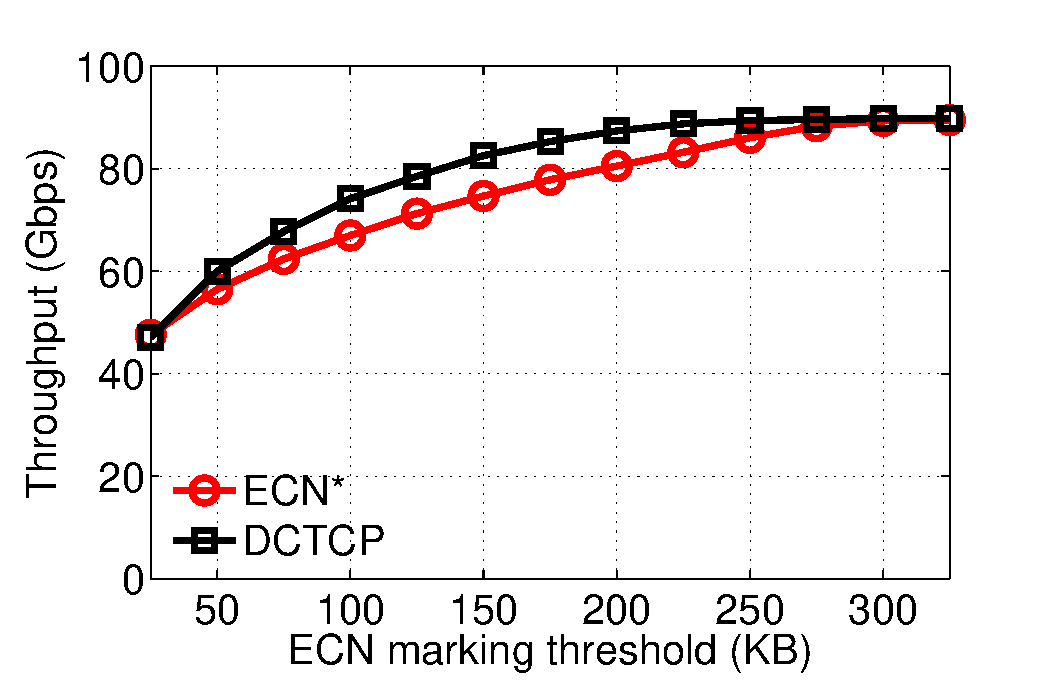
\includegraphics[width=0.75\linewidth]{figs/throughput_ecn_threshold.eps}
      \vspace{-1.5mm}
  \caption{[Testbed] Aggregate TCP throughput with different ECN/RED marking thresholds}\label{fig:throughput_ecn_thresh}
    \vspace{-4mm}
\end{figure}
\begin{table*}[t]
\small
\centering
\begin{tabular}{|l|l|l|l|l|}
\hline
ASIC & Broadcom 56538 & Broadcom Trident+ & Broadcom Trident \uppercase\expandafter{\romannumeral2} & Broadcom Tomahawk \\\hline
Capacity (ports $\times$ BW) & 48 p $\times$ 1 Gbps & 48 p $\times$ 10 Gbps & 32 p $\times$ 40 Gbps & 32 p $\times$ 100 Gbps \\\hline
Total buffer             & 4MB   & 9MB  & 12MB & 16MB (4 MMUs) \\\hline
Buffer per port          & 85KB  & 192KB  & 384KB & 512KB \\\hline
Buffer per port per Gbps & 85KB  & 19.2KB & 9.6KB & 5.12KB \\\hline
\end{tabular}
%\vspace{-2mm}
\caption{Information of some commodity datacenter switching chips. Note that Tomahawk has 4 switch cores, each with its own MMU and 4MB buffer~\cite{tomahawk_buffer1,tomahawk_buffer2}. Dynamic buffer sharing only happens within the single core.}
\label{tab:chip_buffer}
\vspace{-2mm}
\end{table*}
Figure~\ref{fig:throughput_ecn_thresh} shows aggregate throughput results with different thresholds.
As expected, ECN$^{*}$ starts to achieve 100\% throughput on 325KB which is close to the bandwidth-delay product (BDP) in our testbed. Our measurement also shows that DCTCP performs similar as ECN$^{*}$ in practice. The minimum ECN marking threshold that DCTCP requires for 100\% throughput is 250KB. The reader may be curious that why our experiment observation of DCTCP seems inconsistent with theory results in~\cite{dctcp-analysis} (0.17BDP buffering is enough for 100\% throughput). We think this is mainly due to packet bursts that are caused by various interactions between the OS and the NIC (\eg, TSO, GRO and interrupt moderation). Hence, a much larger ECN marking threshold is required to absorb bursts. Such complex burst behaviors are difficult to capture by ideal fluid model in~\cite{dctcp-analysis}, thus resulting in the theory-practice gap\footnote{Such performance-theory gap has also been identified by previous work~\cite{tuning} and even DCTCP paper itself~\cite{dctcp}.}. We also conduct the above experiment using Windows Server 2012 R2 and observe that DCTCP requires $\sim$60-70\% BDP buffering for 100\% throughput.

\vspace{-1mm}
\parab{Production Datacenters:}Compared to our simple small-scale testbed, production datacenters are more challenging and have larger base latency. At the end host, packets may experience high processing delay due to kernel scheduling. In the network, packets experience innegligible processing delay when going through various middleboxes (\eg, firewall, IPSec gateway and load balancer). Long-distance cables and multiple switch hops also bring several-microsecond delay. Above factors greatly increase the actual latency in production environments. In~\cite{pingmesh}, the authors show that even the 50th percentile inter-pod latency can exceed 200$\mu$s. Such latency eventually transfers to a large buffer demand. Consider a 100Gbps network with 80$\mu$s base RTT, the per-port buffer requirement of ECN$^{*}$ can easily reach 1MB.

\subsection{Buffer becomes increasingly insufficient}\label{sec:buffersize}
However, the buffer size of commodity switching chips does not increase as expected. We list buffer and capacity information of some commodity chips in Table~\ref{tab:chip_buffer}. The capacity significantly outpaces the buffer size, resulting in decreasing buffer per port per Gbps (from 85KB to 5.12KB). The reasons of shallow switch buffers are at least two-fold.
\begin{ecompact}
\item The memory used in switch buffers is high-speed SRAM. Compared to DRAM, SRAM is more expensive as it requires more transistors.
\vspace{-1mm}
\item The area increases with the memory size. When the area becomes large, the read/write latency will increase, making the memory access speed hard to match the link speed.
\end{ecompact}
Therefore, most commodity switches in DCNs are shallow buffered. We envision that such trend will hold for future 200/400Gbps switching chips.

\section{Problems caused by extremely shallow buffer}\label{sec:problem}
In this section, we show that, in extremely shallow-buffered high-speed DCNs, existing TCP/ECN solutions use switch buffers either (1) too aggressively, thus causing excessive packet losses at high loads ($\S\ref{subsec:buffer-aggressive}$) or (2) too conservatively, thus seriously degrading throughput at low loads ($\S\ref{subsec:buffer-conservative}$).

\subsection{Standard ECN configuration causes excessive packet losses}\label{subsec:buffer-aggressive}
To achieve 100\% throughput, operators need to configure a moderate marking threshold (\eg, $C\times RTT \times \lambda$). To the best of our knowledge, this is current operation practice in many production DCNs. However, the standard ECN configuration is likely to overfill extremely shallow buffers when many ports are congested simultaneously. Therefore, it may cause excessive packet losses and poor performance for small flows.

We take Broadcom Tomahawk with 16MB buffer and 32 100Gbps ports as an example. If TCP desires 1MB ($100Gbps\times 80\mu s$) marking threshold per port, the buffer will be overfilled when more than half of the total ports are congested. What is worse, Tomahawk has 4 switch cores to achieve desired performance at the high-speed. Each core has its own MMU and 4MB buffer~\cite{tomahawk_buffer1,tomahawk_buffer2} and dynamic buffer sharing only happens within the single core. Therefore, the buffer of a Broadcom Tomahawk chip will be overfilled when more than 4 ports attached to a single core are congested simultaneously.

\subsection{Conservative ECN configuration degrades throughput}\label{subsec:buffer-conservative}
Realizing the above limitation, a straight forward solution is to configure a lower marking threshold (\eg, $\leq$ average per-port buffer), thus leaving headroom to reduce packet losses. However, this conservative ECN configuration causes much \emph{unnecessary} bandwidth wastage when few ports are congested simultaneously. For example, when only a single switch port is congested, this method still throttles TCP throughput despite the sufficient switch buffer resource.





\section{Solution}\label{sec:design}
%\vspace{-2mm}
\subsection{Design Goals}\label{subsec:design_goals}
We seek to achieve both high throughput and low packet loss rate simultaneously. However, as shown in $\S\ref{sec:problem}$, it is difficult to achieve both metrics when many ports are active simultaneously. When a conflict arises between the two metrics, we prefer to keep low packet loss rate at the cost of sacrificing a small amount of throughput. This is because the bandwidth is generally plentiful in datacenters, while a small increase in packet loss rate (\eg, $\geq0.1\%$) can seriously degrade the application performance and in turn, operator revenue~\cite{timely}. Furthermore, our solution should work with existing commodity switches and legacy network stacks.
%Modifying switch hardware is especially problematic as a new switch ASIC typically takes years to design and implement.

\subsection{\sys Mechanism}\label{subsec:mechanism}
\begin{table}[t]
\small
\centering
\begin{tabular}{|C{1.5cm}|C{6cm}|}
\hline
Parameter & Description\\ \hline
$B$ &  Switch shared buffer size\\ \hline
$N$ &  Total number of switch egress queues \\ \hline
$C$ &  Capacity of the switch queue \\ \hline
$RTT$ & Base round-trip time \\ \hline
$\alpha$ & Parameter for shared buffer allocation\\ \hline
$B_{R}$ & Minimum per-queue required buffer for high throughput and low packet loss rate\\ \hline
$K_{min}$ & Minimum marking threshold for shared buffer ECN/RED\\ \hline
$K_{max}$ & Maximum marking threshold for shared buffer ECN/RED\\ \hline
$P_{max}$ & Maximum marking probability for shared buffer ECN/RED\\ \hline
$h$ & See Equation~\ref{eq:k_min}\\ \hline
\end{tabular}
\vspace{+1mm}
\caption{Shared buffer model parameters}\label{tab:parameter}
\vspace{-5mm}
\end{table}
\begin{table}[t]
\centering
\small
\begin{tabular}{|C{1.5cm}|C{6cm}|}
\hline
Variable & Description\\ \hline
$t$ & Time\\ \hline
$Q_{i}(t)$ & Length of switch queue $i$ at time $t$\\ \hline
$T(t)$ & Queue length control threshold at time $t$\\ \hline
\end{tabular}
\vspace{+1mm}
\caption{Shared buffer model variables}\label{tab:variable}
\vspace{-6mm}
\end{table}
We model the switch as a shared-buffer output-queued switch. Variables and parameters used in the model are listed in Table~\ref{tab:parameter} and~\ref{tab:variable}. We start from the simplest assumption that each switch port only contains a single egress queue\footnote{In $\S\ref{subsec:mechanism}$ and $\S\ref{subsec:parameter}$, we use queue and port interchangeably.} and no buffer is reserved for each queue. Hence, all buffers are dynamically allocated from a single shared buffer pool. The switch has $B$ (shared) buffer space and $N$ egress queues in total. An ECN-based transport~\cite{dctcp,tuning,d2tcp,l2dct} is enabled at the end host. The standard ECN setting has been configured on each port/queue to achieve 100\% throughput.

Today's commodity switching chip typically use Dynamic Threshold (DT) algorithm~\cite{dt} for dynamic buffer allocation. The shared buffer allocated to a queue is controlled by a parameter $\alpha$. At time $t$, the MMU will compute a threshold $T(t)$ to limit the queue length. $T(t)$ is actually a function of the unused shared buffer size and $\alpha$ as follows:
\vspace{-2mm}
\begin{equation}
\vspace{-1mm}
T(t)=\alpha\times(B-\displaystyle\sum_{i=1}^{N} Q_{i}(t))\label{eq:dt}
\vspace{-1mm}
\end{equation}
A packet arriving in queue $i$ at time $t$ will get dropped if $Q_{i}(t)\geq T(t)$. As analyzed in~\cite{dt}, if there are $M$ active queues, each queue can eventually get $\alpha\times B/(1+M\times \alpha)$ buffer space. The more active queues we have, the smaller buffer space each queue can get from the shared pool. $\alpha$ values are typically powers of two for hardware implementation simplicity (\eg, 1/128 to 8 in Tomhawk).

We assume that our ECN-based transport protocol requires at least $B_R$ buffer space per queue to achieve both high throughput and low packet loss rate. We simply treat $B_R$ as a known constant here and show how to determine $B_R$ later in $\S\ref{subsec:parameter}$. When $T(t) > B_R$, it means that the switch has sufficient buffer space to achieve both goals simultaneously. Hence, \sys just marks packets like the standard ECN configuration without degrading throughput.

When $T(t) \leq B_R$, it indicates that the shared buffer pool is highly utilized by many concurrently active ports. In such scenarios, only relying on standard ECN configuration may cause excessive packet losses as analyzed in $\S\ref{subsec:buffer-aggressive}$. Hence, \sys throttles the shared buffer occupancy to avoid excessive packet losses. By Equation~\ref{eq:dt} and $T(t)\leq B_R$, we derive that
\vspace{-2mm}
\begin{equation}
\vspace{-1mm}
\displaystyle\sum_{i=1}^{N} Q_{i}(t)\geq B-B_{R}/\alpha\label{eq:shared_buffer}
\vspace{-1mm}
\end{equation}
%\vspace{-3mm}
Here $\displaystyle\sum_{i=1}^{N} Q_{i}(t)$ is the occupancy of the shared buffer pool at time $t$, and $B$, $B_{R}$ and $\alpha$ are all known parameters. This implies that, to prevent excessive packet losses, \sys should throttle the shared buffer occupancy from exceeding a static threshold $B-B_{R}/\alpha$.

To realize this, we leverage the shared buffer ECN/RED functionality which has been widely supported in commodity switching chips~\cite{arista_ecn,mqecn}. Shared buffer ECN/RED follows the original RED algorithm~\cite{RED} but tracks the occupancy of a shared buffer pool to mark packets. It can effectively control shared buffer occupancies. Moreover, shared buffer ECN/RED can be used in combination with other switch ECN configurations. When several ECN configurations coexist, a packet gets marked if anyone decides to mark it first.

%\vspace{-1mm}
\parab{Summary:}\sys is built on top of existing ECN-based transports and per-port standard ECN configuration. It further enables shared buffer ECN/RED at the switch to achieve buffer-aware congestion control.
\vspace{-1mm}
\begin{icompact}
\item When few ports are active, the shared buffer resource is abundant and per-port standard ECN configuration will take effect first to strike the balance of high throughput and low latency as before~\cite{dctcp}. Both high throughput and low packet loss rate can be achieved.
\vspace{-1mm}
\item When more and more ports become congested, the shared buffer resource turns scarcer. Shared buffer ECN/RED will be automatically triggered first to prevent packet losses at the cost of sacrificing a small amount of bandwidth.
\vspace{-1mm}
\end{icompact}

\subsection{Parameter Selection}\label{subsec:parameter}
We now derive several parameters for \sys. First, we determine $B_R$, the minimum per-queue (port) buffer size for both high throughput and low packet loss rate. With $B_R$ fixed, we then decide marking thresholds and probability of shared ECN/RED. Note that in this section we give several useful rules-of-thumb to set parameters while leaving optimal parameter settings for future work.

\vspace{-1mm}
\parab{Determine $B_R$:}Statistics has shown that there is typically a small number of concurrent large flows to the same receiver in DCNs~\cite{dctcp}. Hence, we consider a simple scenario where several synchronized long-lived flows share a bottleneck link. $C\times RTT\times \lambda$ per port buffering is required for 100\% throughput. Furthermore, the lag in ECN control loop imposes extra buffer requirement to avoid packet losses. When a packet gets ECN marked at switch egress\footnote{Modern shared buffer switches mark packets at egress side~\cite{ecn_or_delay}.}, the sender will reduce its window after one $RTT$. During this $RTT$ interval, extra buffer space is required to absorb the queue increase. We consider the most challenging slow start phase. As an ACK packet can trigger two MTU-sized data packets, the aggregate sending rate reaches $2C$ and the switch queue gradient is $C$. Therefore we need $C\times RTT$ extra buffer space to avoid packet losses and $C\times RTT\times (1+\lambda)$ buffer space in total to achieve both goals. Through ns-2 simulations, we confirm that $C\times RTT\times (1+\lambda)$ also works well for a mix of small and large flows. As $C$ and $\lambda$ are both known and $RTT$ can be measured~\cite{pingmesh,tuning} in production DCNs, operators can easily compute the value of $B_R$.

\vspace{-1mm}
\parab{Determine parameters for shared buffer ECN/RED:}We leverage shared buffer ECN/RED to prevent the shared buffer occupancy from exceeding $B-B_{R}/\alpha$. To achieve fast reaction to bursty traffic, we mark packets based on the instantaneous buffer occupancy. Shared buffer ECN/RED has 3 parameters to configure: minimum threshold $K_{min}$, maximum threshold $K_{max}$ and maximum probability $P_{max}$. When the buffer occupancy is: 1) below $K_{min}$, no packet is marked; 2) between $K_{min}$ and $K_{max}$, packets are marked according to a probability; 3) exceeds $K_{max}$, all packets get marked.

Inspired by  DCTCP~\cite{dctcp}, our first choice is to set $K_{min}=K_{max}\leq B-B_{R}/\alpha$, in which only a single threshold is required. However, with such cut-off setting, all flows sharing a buffer pool are likely to reduce their window at the same time, resulting in global synchronization problem and a further loss of throughput~\cite{RED}.

Therefore, we decided to perform a probabilistic marking by setting $K_{min}<K_{max}=B-B_{R}/\alpha$. The key here is to control the range between $K_{min}$ and $K_{max}$. A too small $K_{max}-K_{min}$ will make buffer occupancy regularly ramp up beyond $K_{max}$, still causing global synchronization and even packet losses. As original RED work~\cite{RED} suggests, $K_{max}-K_{min}$ should be made sufficiently large (\eg, larger than typical increase in the shared buffer occupancy during a RTT) to avoid global synchronization. Hence, the choice of $K_{max}-K_{min}$ depends on both the number of ports $N$ and link capacity $C$. In \sys, we set $K_{min}$ as follows:
\vspace{-3mm}
\begin{equation}
\vspace{-1mm}
\displaystyle K_{min}=B-B_{R}/\alpha-C\times N\times h\label{eq:k_min}
\vspace{-1mm}
\end{equation}
where $h$ is a parameter to control $K_{max}-K_{min}$. In our evaluation, we set $h$ to 8$\mu$s. For the maximum marking probability $P_{max}$, we set it to 10\% according to~\cite{RED}.

\subsection{Discussion}\label{subsec:discussion}
\vspace{-1mm}
\parab{Impact of multiple MMUs:}Each MMU has its own shared buffer ECN/RED without interfering with each other. Hence, \sys supports multi-MMU chips.

\vspace{-1mm}
\parab{Impact of different $\alpha$ values:}Operators may configure different $\alpha$ values for different queues for differentiated network services. In such scenarios, we can choose the minimum value $\alpha_{min}$ among them and update shared buffer ECN/RED parameters as follows: $K_{max}=B-B_{R}/\alpha_{min}$, $K_{min}=B-B_{R}/\alpha_{min}-C\times N\times h$.

\vspace{-1mm}
\parab{Impact of static reserved buffers:}When both static reserved buffers and dynamic shared buffers exist, the MMU first tries to use static reserved buffers. Therefore, we should reduce $B_R$ to incorporate the static reserved buffer into \sys. Let $S_{min}$ denote the minimum static buffer size reserved for a single queue. Our recommended value for $B_R$ should become $C\times RTT\times (1+\lambda)-S_{min}$





\begin{figure*}[t]
\centering
\begin{minipage}{0.245\linewidth}
   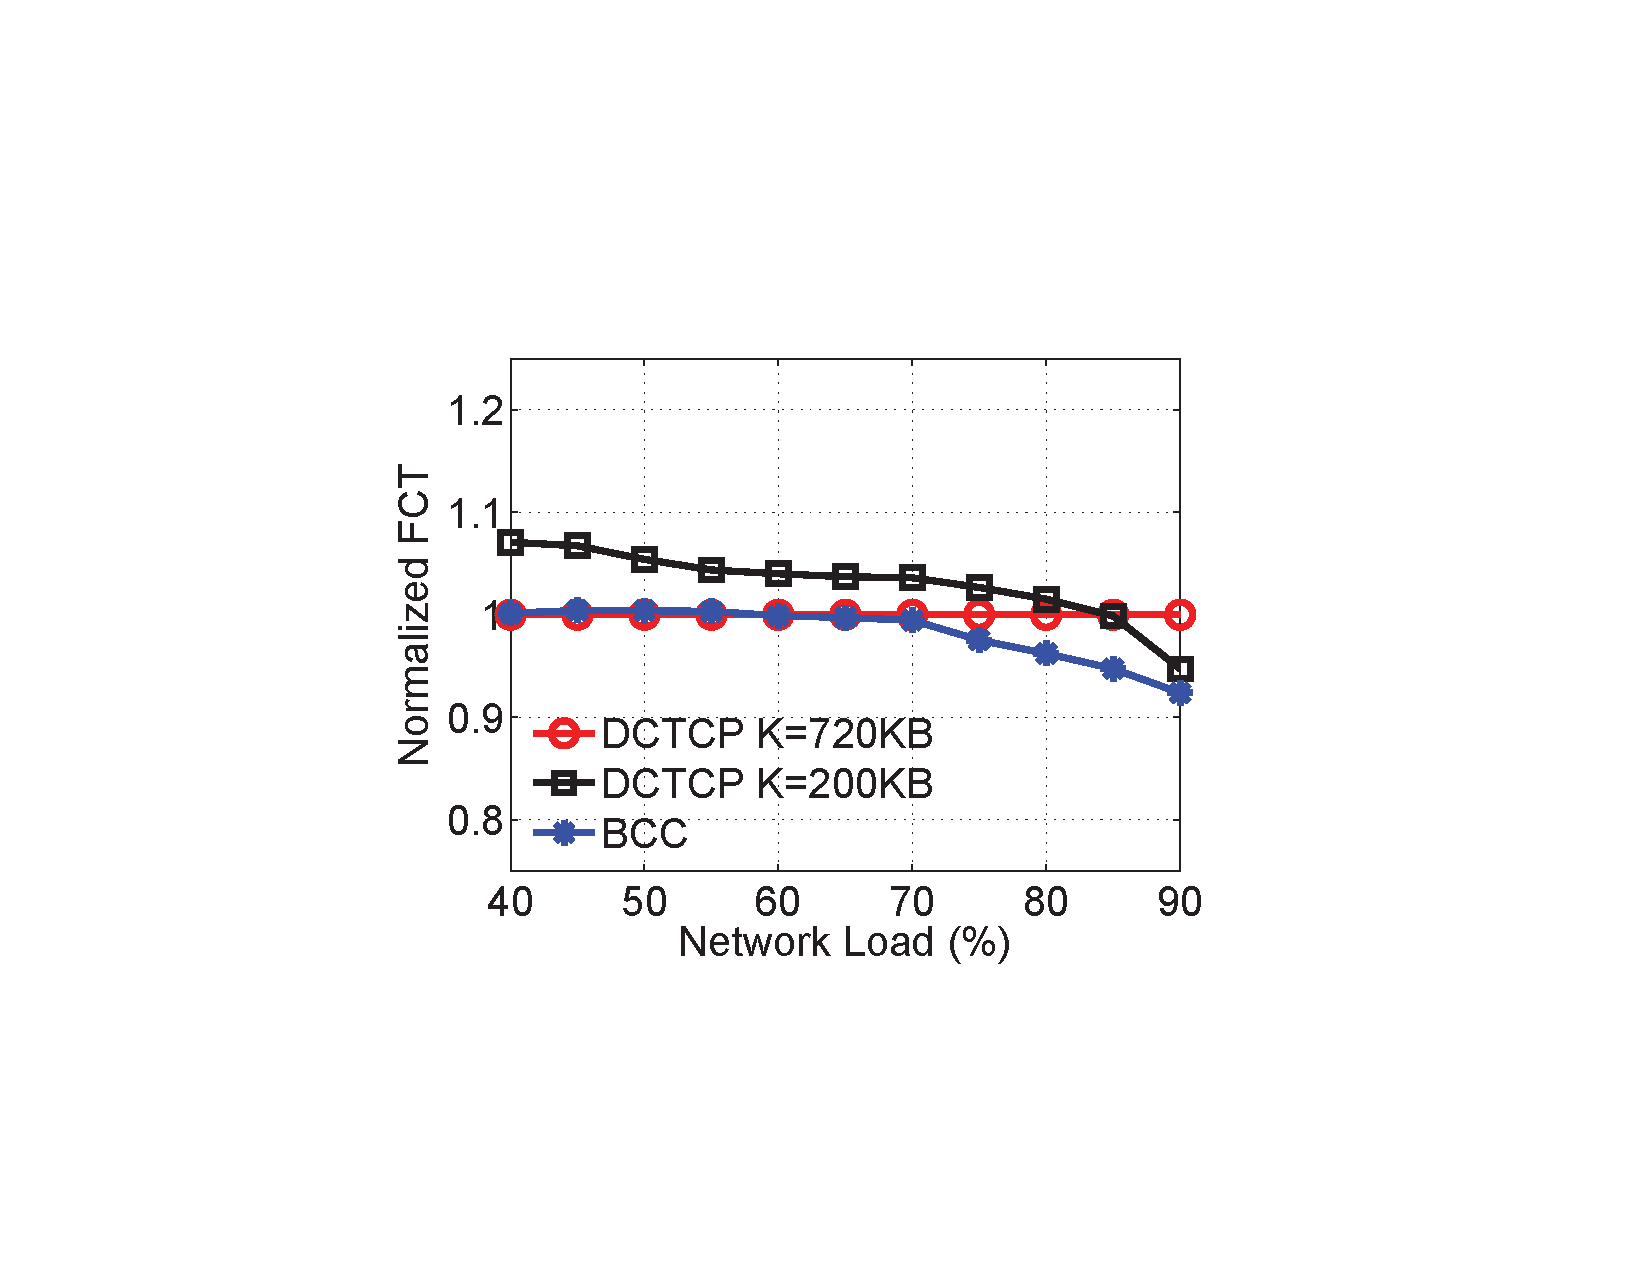
\includegraphics[width=1\linewidth]{figs/websearch_overall_avg_fct.pdf}
   \centerline{(a) Overall: Avg}
\end{minipage}
\begin{minipage}{0.245\linewidth}
   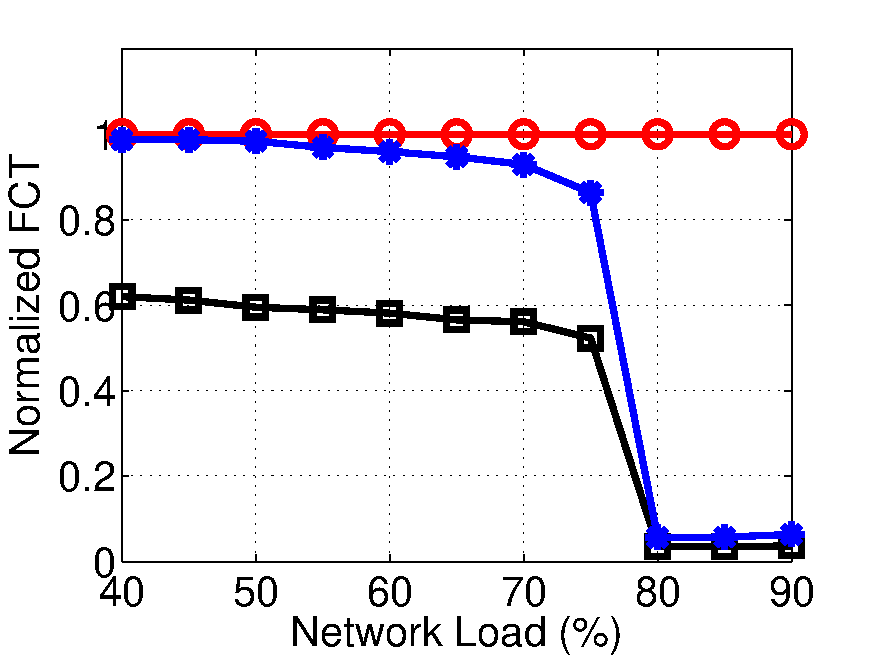
\includegraphics[width=1\linewidth]{figs/websearch_small_tail_fct.pdf}
   \centerline{(b) (0,100KB]: 99th percentile}
\end{minipage}
\begin{minipage}{0.245\linewidth}
   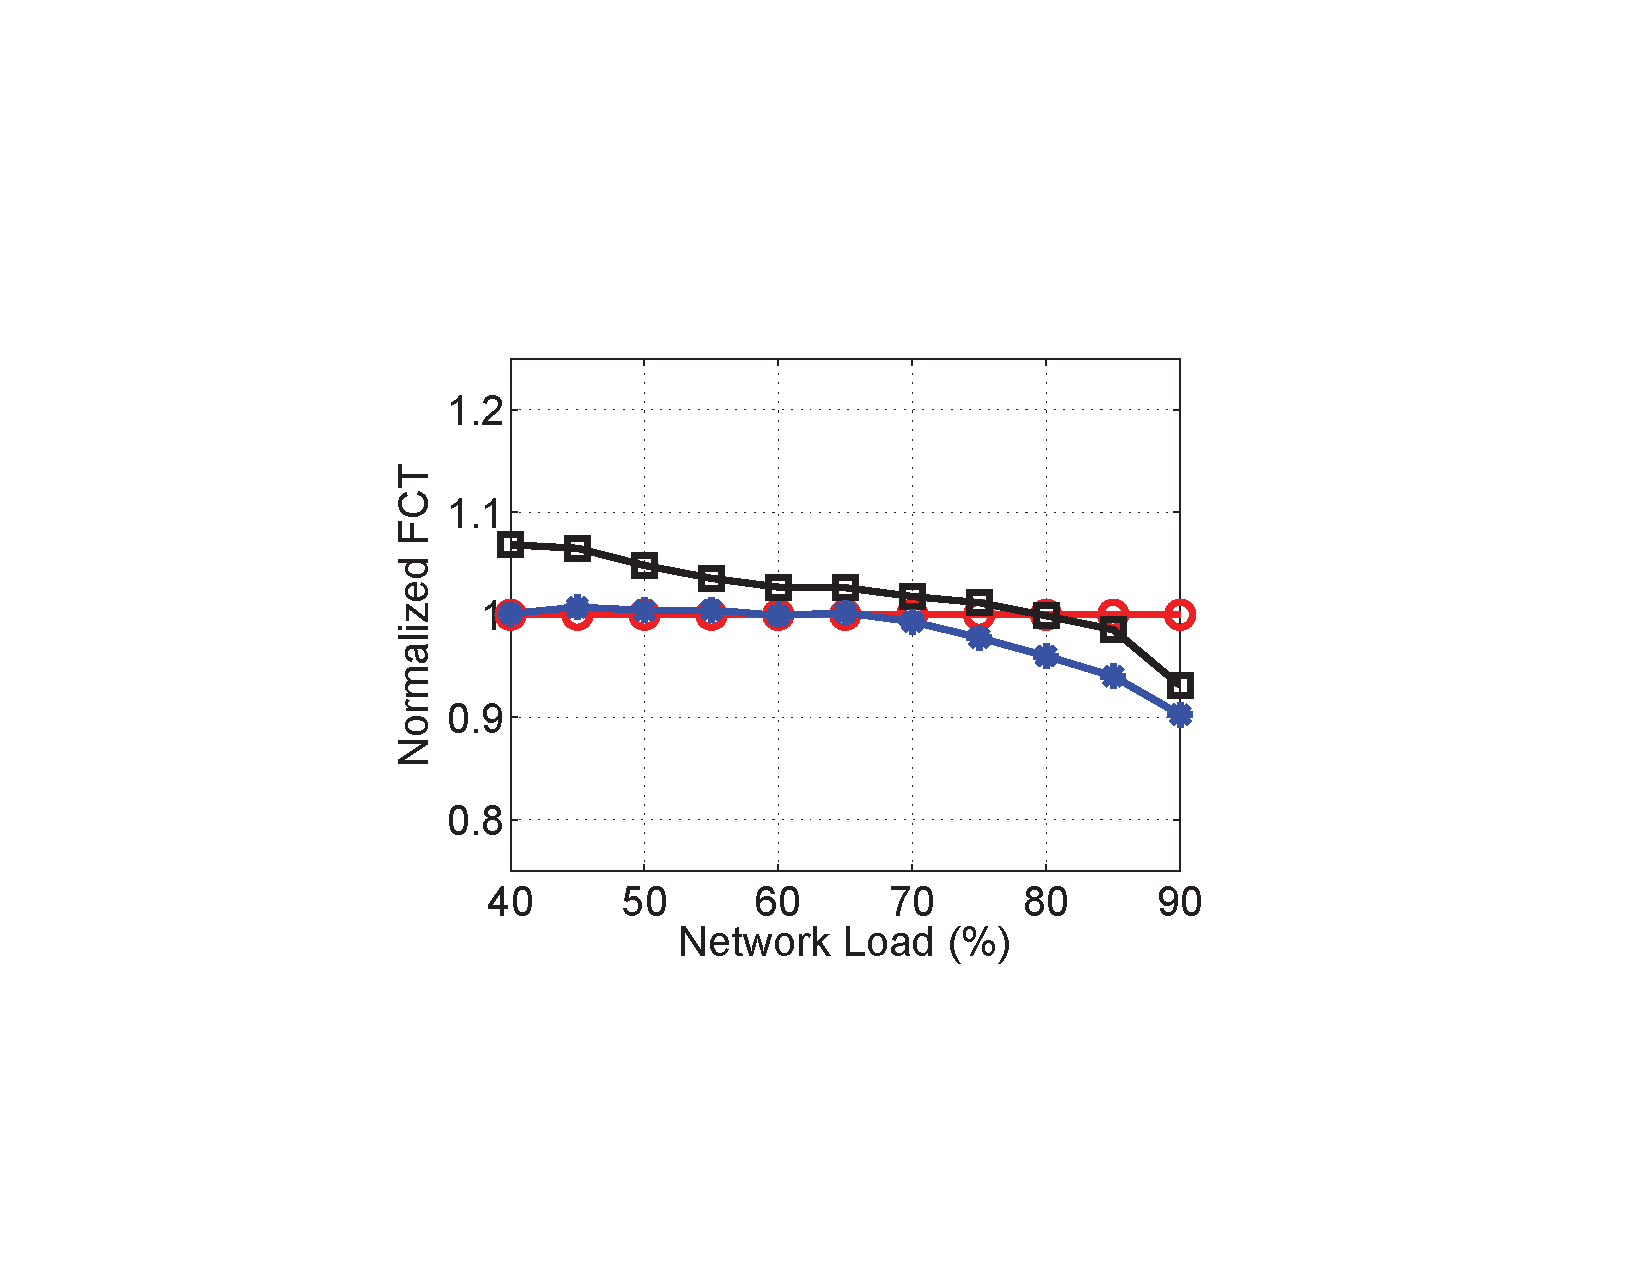
\includegraphics[width=1\linewidth]{figs/websearch_medium_avg_fct.pdf}
   \centerline{(c) (100KB,10MB]: Avg}
\end{minipage}
\begin{minipage}{0.245\linewidth}
   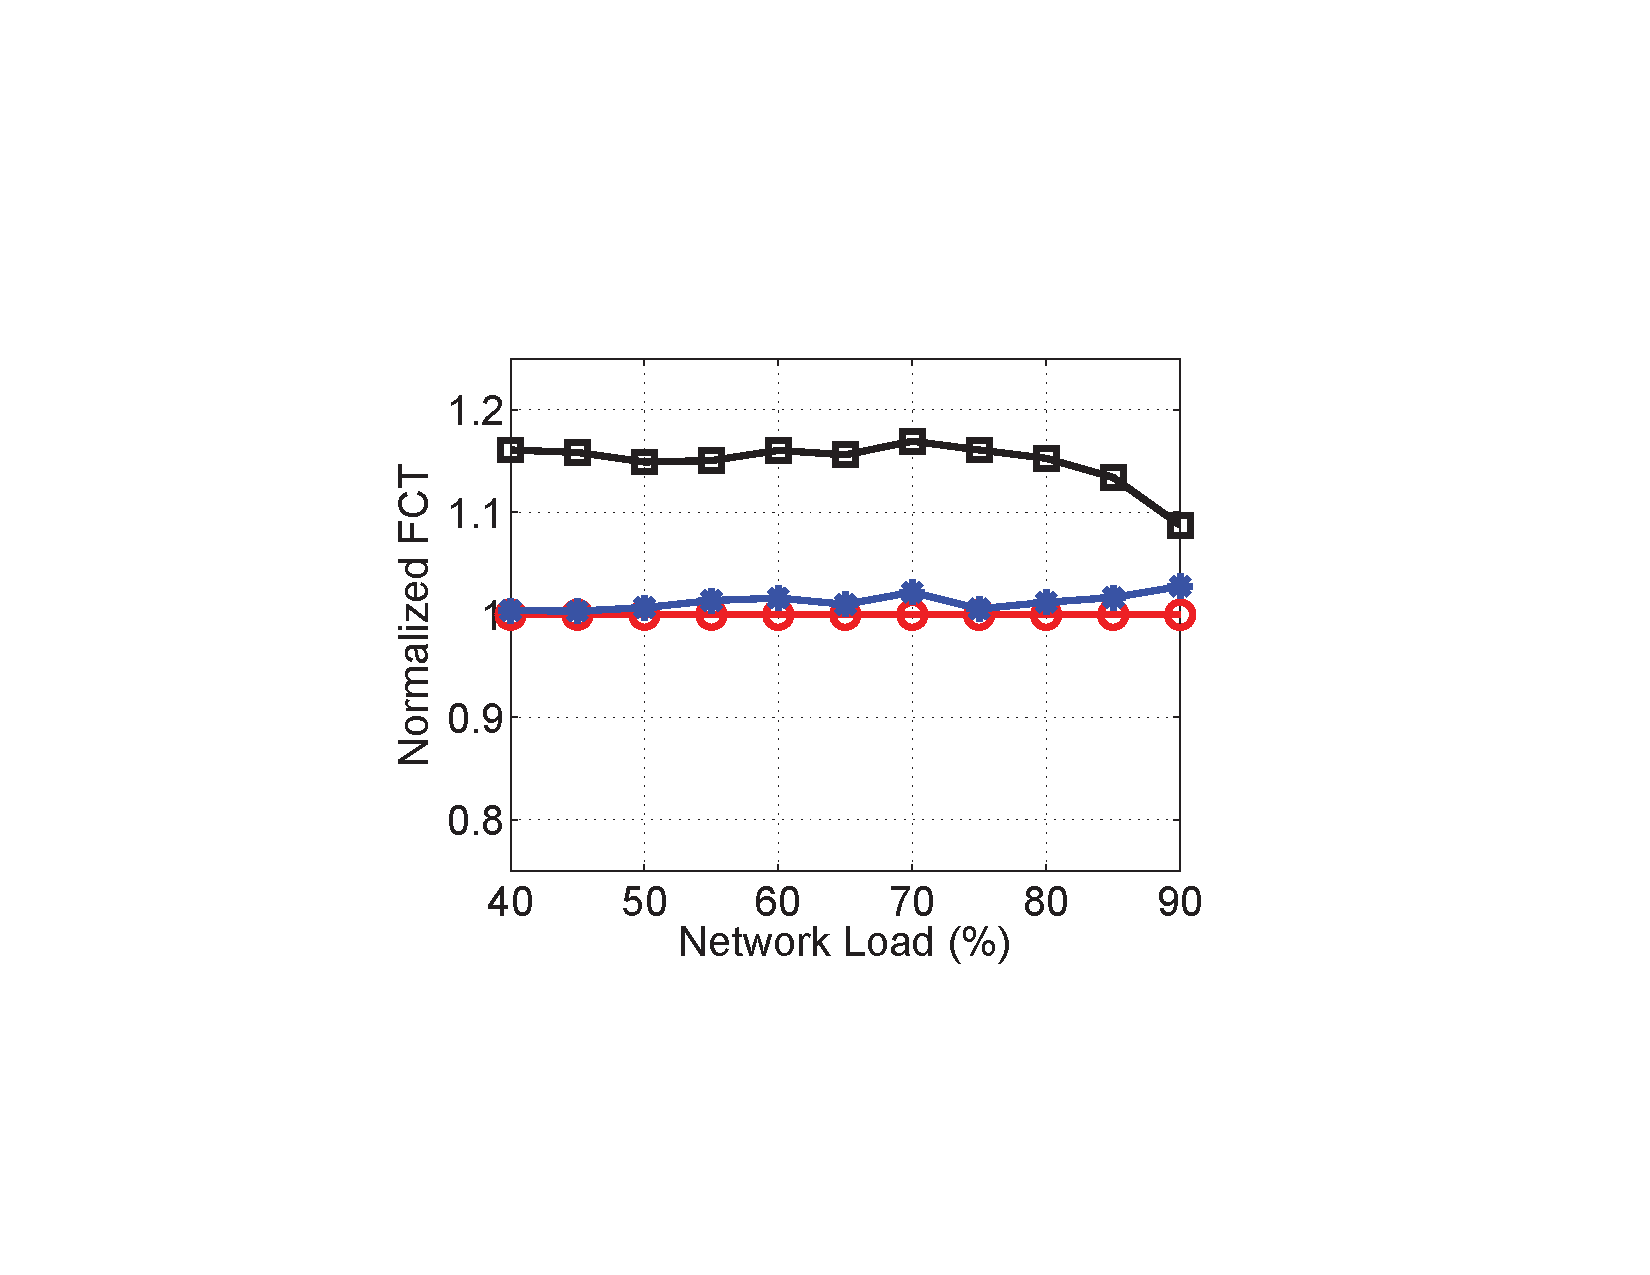
\includegraphics[width=1\linewidth]{figs/websearch_large_avg_fct.pdf}
   \centerline{(d) (10MB,$\infty$): Avg}
\end{minipage}
  \vspace{-2mm}
\caption{[Simulation] Flow Completion Time (FCT) results for the web search workload. Results are normalized to values achieved by DCTCP K=720KB for clear comparison.}\label{fig:websearch_fct}
  \vspace{-3mm}
\end{figure*}
\section{Evaluation}\label{sec:evaluation}
In this section, we present ns-2 simulations results.

\vspace{-1mm}
\parab{Topology:}We simulate a 128-host 100Gbps leaf-spine topology with 8 leaf switches and 8 spine switches. We use ECMP for load balancing. The base fabric RTT is $\sim$80$\mu$s. The BDP is 1MB. The jumbo frame is enabled.

\vspace{-1mm}
\parab{Workload:}We generate traffic according to the web search workload (see~\cite{dctcp} for more details about the distribution). We adjust the flow arrival intervals to achieve the desired load in the network core.

\vspace{-1mm}
\parab{Buffer:}To emulate Tomahawk chip, we attach every 8 switch ports to a 3MB shared buffer pool. We set $\alpha$ to 4 for all ports. In addition, each switch port has 128KB static reserved buffer. We allocate 10MB buffer for each NIC at the host.

\vspace{-1mm}
\parab{Schemes compared:}We use DCTCP~\cite{dctcp} and set RTOmin to 5ms. We compare the following three schemes:
\begin{icompact}
\vspace{-1mm}
\item \textbf{DCTCP K=720KB}: This is a standard ECN configuration (current practice). We configure the per-port (queue) ECN/RED marking threshold to 720KB (0.72BDP based on $\S\ref{subsec:buffer_requirement_high_speed}$) for 100\% throughput.
\vspace{-1mm}
\item \textbf{DCTCP K=200KB}: We configure the per-port (queue) ECN/RED marking threshold to 200KB, which is smaller than average per-port buffer size (512KB), to reduce packet losses.
\vspace{-1mm}
\item \textbf{\sys}: \sys requires two ECN configurations at the switch. We set per-port (queue) ECN/RED marking threshold to 720KB like the standard ECN configuration. Since $\lambda$ is 0.72 for DCTCP and the per-port static reserved buffer size $S_{min}$ is 128KB, $B_R=C\times RTT\times(1+\lambda)-S_{min}\approx$1.6MB. Therefore, $K_{max}\approx$2.6MB, $K_{min}=K_{max}-C\times N\times h\approx$1.8MB and $P_{max}$=10\%.
\end{icompact}

\vspace{-2mm}
\parab{Performance metrics:}We use flow completion time (FCT) as the performance metric and breakdown FCT results across small (0,100KB], medium (100KB,10MB] and large (10MB,$\infty$) flows. Since the performance of many real-time applications depends on the slowest flow, we consider the 99th percentile FCT for small flows.

\vspace{-1mm}
\parab{Result analysis:}According to Figure~\ref{fig:websearch_fct}, we have the following two key observations.
%\vspace{-1mm}
\begin{ecompact}
\vspace{-1mm}
\item At low loads, \sys performs similar as K=720KB while generally outperforming K=200KB, especially for medium and large flows. With the sufficient buffer resource, \sys can fully utilize the link capacity without triggering shared buffer ECN/RED. By contrast, K=200KB still conservatively marks packets, thus significantly degrading throughput. Compared to K=200KB. \sys achieves up to $\sim$13.5\% (6362$\mu$s to 5503$\mu$s) lower average FCT for large flows. K=200KB only shows some performance advantage ($\sim$100$\mu$s) on small flows, due to its lower switch queueing.
\vspace{-1mm}
\item At high loads, \sys generally outperforms the other two schemes. For small flows, \sys achieves up to  94.4\% (5174$\mu$s to 291$\mu$s) lower 99th FCT compared to K=720KB. This is because K=720KB causes excessive packet losses due to the exorbitant shared buffer utilization. The packet loss rate with K=720KB exceeds 0.3\% at 90\% load. This results in frequent TCP timeouts, which seriously increases FCT by at least 5ms (RTOmin). By contrast, at 90\% load, the packet loss rate with \sys is lower than 0.08\%.

    For large flows, \sys's performance is within $\sim$0.4-2.8\% of the K=720KB. This suggests that \sys only slightly degrades large flows. We think that the lower packet loss rate with \sys can make up for throughput loss to some degree. By contrast, DCTCP K=200KB is still so conservative that it increases FCT by at least $\sim$9\% compared to K=720KB.
\end{ecompact}
%In summary, \sys can operate based on the real-time shared buffer utilization, thus keeping good performance in various scenarios.



\section{Related Work}\label{sec:related}
\vspace{-1mm}
\parab{Bufferless Transports in DCNs:}There are some bufferless transport designs in DCNs. But they may encounter various deployment challenges. PDQ~\cite{pdq} requires non-trivial modifications to switch hardware. Fastpass~\cite{fastpass} and Flowtune~\cite{flowtune} leverage a centralized scheduler, which is easy to suffer from failures and poor scalability. pHost~\cite{phost} relies on the congestion free network core, which does not hold for many DCNs. By contrast, \sys is easy to deploy with only one more ECN configuration at commodity switches.

\vspace{-1mm}
\parab{PFC:}PFC (Priority-based Flow Control)~\cite{pfc} has been enabled in some DCNs to achieve lossless networks~\cite{rdma_scale}. PFC needs to reserve enough buffer space as the headroom~\cite{rdma_scale}. The size of the headroom is greatly affected the propagation delay. Deploying PFC in large-scale DCNs results in very large headroom size, which may not be affordable for commodity switches. Therefore, PFC is still limited in modest scale (\eg. thousands of servers). Even so, commodity switches can still only support a small number (\eg, 2) of lossless traffic classes~\cite{rdma_scale}. Moreover, PFC may introduce deadlock problem, causing damage to the whole network~\cite{rdma_scale}. 
%\vspace{-0.2in}
\section{Conclusion}\label{sec:conclusion}
%In production DCNs, the great increase of the link speed significantly outpaces the slow increase of the switch buffer, resulting in extremely shallow-buffered DCNs. To address it, we have proposed \sys, a simple yet effective solution with only one more shared buffer ECN/RED configuration at commodity switches. \sys operates based on real-time shared buffer utilization. It maintains low packet loss rate persistently while only slightly degrading throughput when the buffer becomes insufficient. We validated BCC¡¯s efficacy in a 100G testbed and demonstrated its superior performance using extensive simulations.

In production DCNs, the increase of link speed significantly outpaces the increase of switch buffer size, resulting in an extremely shallow-buffered environment. Consequently, prior TCP/ECN solutions suffer from severe performance degradation. To address it, we introduced \sys, a simple yet effective solution with only one more shared buffer ECN/RED configuration at commodity switches. \sys maintains low packet loss rate persistently while only slightly degrading throughput when the buffer becomes insufficient. We demonstrated its superior performance using extensive simulations. 



\bibliographystyle{ACM-Reference-Format}
\bibliography{reference}

\end{document}
